\documentclass[12pt,a4paper]{article}
\usepackage[utf8]{inputenc}
\usepackage[spanish]{babel}
\usepackage{textcomp}
\usepackage{graphicx}
\usepackage{url}
\usepackage[nottoc,numbib]{tocbibind}
\graphicspath{ {./images/} {./images2/} }
\usepackage[left=2cm,right=2cm,top=3cm,bottom=2cm]{geometry}
\author{Mario Arguello Borge, Josué Céspedes Miranda}
\title{Proyecto 0}
\begin{document}
\begin{titlepage}
\begin{center}
\begin{large}
UNIVERSIDAD NACIONAL COSTA RICA \\
\begin{figure}[htp]
\centering

\includegraphics[width=4cm]{imagenes/240px-UNA.png} 
\label{foto}
\end{figure}
\end{large}
\begin{large}
Facultad de Ciencias Exactas y Naturales
\end{large} 
\begin{large}
\vspace*{1cm}\\
Curso:\\
\vspace*{2mm}
Paradigmas de Programación\\
\end{large}
\vspace*{8mm}
\begin{large}
\textbf{Proyecto 1: 
NQueens
}\\
\end{large}
\begin{figure}[htp]
\centering
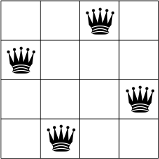
\includegraphics[width=4cm]{imagenes/queens.png} 
\end{figure}
\begin{large}
\vspace*{1cm}
Profesor:\\
\vspace*{5mm}
Eddy Miguel Ramírez\\
\end{large}
\begin{large}
\vspace*{1cm}
Estudiantes: \\
\vspace*{5mm}
Mario Arguello Borge \\
Josué Céspedes Miranda \\
\end{large}
\vspace*{1cm}
II CICLO\\
\vspace*{1cm}
2020
\end{center}
\end{titlepage}
\tableofcontents
\pagebreak
\section{Resumen ejecutivo}
\bigskip
 El presente trabajo esta realizado con el objetivo de hacer un uso práctico de distintos modelos con el fin de brindar una solución al popular problema NReinas bajo el uso de un paradigma funcional, que permita conocer nuevos conceptos y permita establecer diferentes perspectivas a la hora de brindar soluciones a distintos problemas mediante programación. \\
 	
 El problema de NReinas es un acertijo con bastante popularidad, propuesto por el ajedrecista alemán Maxx Bezzel en 1848, consiste en colocar N reinas en un tablero con dimensiones NxN, su principal desafío radica en colocar las N reinas, mencionadas anteriormente, de tal manera que ninguna reina quede atacando otra. Dado que en el ajedrez esta pieza puede atacar a las piezas que se encuentren en su misma fila, misma columna, o en sus respectivas diagonales. \\
 	
 En este documento se detallan dos posibles métodos para dar solución al problema explicado previamente. La primera, y más común a la hora de resolver este algoritmo, es una solución implementando backtracking, la cual se ha diseñado y escrito en Scheme, el cual como se mencionó al inicio tiene características de programación funcional y es un subconjunto del lenguaje de programación LISP; fue desarrollado en el MIT (Massachusetts Institute of Technology). La segunda solución ha sido implementada sobre algoritmos genéticos, se ha trabajado con elitismo y con un porcentaje de mutación de un 5\%, la solución para este caso esta escrita en Erlang, el cual es también es un lenguaje de programación funcional de alto nivel, diseñado en los años 80 en los laboratorios de Ciencias y Computación de la compañía de telefonía sueca Ericsson, y fue diseñado para escribir aplicaciones concurrentes y distribuidas de funcionamiento ininterrupido. \\
 	
 Además, este trabajo pretende plasmar las distintas diferencias presentes en los métodos utilizados para dar solución al problema, establecer una comparación basada en el tiempo de ejecución de cada una de las soluciones y que permita obtener como resultado cual presenta mejores características de desempeño. Por otra parte, ambas soluciones representan una oportunidad para los estudiantes participantes en conocer nuevos paradigmas, poder incursionar en temas de mucho interés como en el caso de algoritmos genéticos que  son temas muy amplios y que lamentablemente es díficil encontrar en un curso dentro del programa de la carrera de Ingeniería en Sistemas de Información en la Universidad Nacional de Costa Rica que abarque la investigación e implementación de este tipo de algoritmos, que se encuentran relacionados a temas de inteligencia artificial y que son utilizados para resolver problemas de búsqueda y optimización, que concuerdan con los parámetros necesarios para dar una solución al problema de NReinas. Por lo que este proyecto representa: 1) un reto, por la parte de investigación y la utilización de un paradigma distinto a la programación orientada a objetos(POO), que incluye un cambio en la forma de pensar, y 2) la oportunidad de aprender temas nuevos y relevantes que pueden llegar a tener un impacto positivo en un futuro profesional. \\
 	
 	Aquí se documentan la descripción de las soluciones, los principales problemas encontrados durante su desarrollo, aprendizajes obtenidos, se adjuntan los resultados de las pruebas efectuadas y demás aspectos concernientes para el proyecto.
 	
\pagebreak
\section{Introducción}

	El presente trabajo tiene como propósito presentar la solución del famoso problema de las n-reinas, el cual consiste en colocar $N $ reinas en un tablero de $NXN $ tal que ninguna de estas pueda ser “atacada” por otra reina y el debido análisis del proceso de resolución, el cual se hará mediante el uso del backtracking y los algoritmos genéticos en dos distintos paradigmas funcionales.

	Para comprender la resolución de este problema es necesario tener en cuenta el concepto de backtracking o “vuelta atrás”, el cual consiste en la búsqueda sistemática de posibles soluciones, donde a partir de un caso base se crean sub-casos  los cuales a su vez son tomados como base para nuevas posibles soluciones expandiéndose hasta encontrar un camino sin salida o una solución apropiada, dado esto ,el algoritmo da un paso hacia atrás con el fin de continuar con el análisis de la siguiente posibilidad. En el caso de los algoritmos genéticos, es una técnica de resolución de problemas que se basa en la evolución biológica, donde se inicia con un conjunto de posibles soluciones denominado población y una métrica llamada función de aptitud que permite evaluar cada posible solución, a partir de esto, se seleccionan los mejores candidatos de la población los cuales generaran otro grupo de posibles soluciones la cual es considerada la “siguiente generación”, este ciclo continua de tal manera que es posible que alguna de las generaciones presente una solución adecuada para el problema.  

	Entre las características mas importantes de la aplicación del backtracking para la resolución de este problema podemos mencionar el hecho de que es capaz de calcular todas las posibles soluciones (a costo de un tiempo mayor de resolución) y su facilidad de implementación, por el lado contrario, el algoritmo genético es capaz de encontrar una única solución  para una cantidad grande de reinas lo que resulta beneficioso sobre el algoritmo de backtracking en estos casos, sin embargo su implementación resulta un poco mas complicada.
\bigskip
\bigskip 


\pagebreak
\section{Marco teórico}
\bigskip
	Como se ha mencionado previamente, para dar solución al problema de NReinas se han utilizado dos lenguajes de programación funcionales. A continuación de profundiza un poco más en la historia, características de Scheme y Erlang y sus principales usos.\\
\begin{enumerate}
 \item  \textbf{Scheme} \\
 	Es un lenguaje de programación de alto nivel, se le considera un lenguaje altamente expresivo. Su sintaxis es fácil de leer pero no lo es tanto comparándolo con Python. Opera sobre estructuras como listas, cadenas, vectores, tuplas y posee conjuntos de datos que lo hacen muy versátil.
 	\begin{itemize}
	\item Historia: surgió en los laboratorios del MIT en 1975, cuando Guy L. Steele y Gerald J. Sussman buscaban un lenguaje con un semántica clara y sencilla. Originalmente se llamaba "Schemer", se le cambió el nombre ya que sus creadores usaban el sistema operativo ITS, que limitaba la longitud del nombre de los ficheros a 6 caracteres.
	\item Antecedentes: altamente influenciado por el cálculo lambda. Su desarrollo ha sido lento, ya que las personas encargadas de su estandarización es muy conservadora y ha sido difícil añadirle nuevas características. Se le considera una de los mejores lenguajes de propósito general. Fue el primer dialecto de Lisp que usó ámbito estático o léxico en lugar de dinámico de forma exclusiva. 
	\item Características: filosofía minimalista, su mecanismo principal para el control de flujo son las llamadas recursivas finales. Además, Scheme ofrece gestión automática de memoria, popularmente conocido como recolector de basura. Las listas son la estructura de datos básica, no hay sintaxis explícita para crear registros o estructuras o para programación orientada a objetos. La programación funcional pura no necesita de variables ni manejo de memoria compartida, por lo que hacen a Scheme una buena opción en presencia de procesos concurrentes. Una de las desventajas es que existen múltiples implementaciones diferentes, cada una utiliza extensiones y bibliotecas propias que se tornan incompatible entre sí.
	\item Usos: la mayoría de uso que se le da a Scheme se refiere a la parte educativa. Profesores de universidad, como es el caso del profesor R. Kent Dybvig que trabaja en la Universidad de Indiana, se concentra en el prototipado de nuevas semánticas para Scheme, incluso tiene a la venta un compilador de Scheme con su colega Daniel P. Friedman. También, hay muchos otros profesores de distintas universidades que lo usan como lenguaje de enseñanza. \\
	
	\end{itemize}
 \item  \textbf{Erlang} \\
 Es un lenguaje de programación funcional de alto nivel, que se ubica también dentro del paradigma de Programación Declarativa, diseñado para escribir aplicaciones concurrentes y distribuidas de funcionamiento ininterrumpido. Erlang cuenta con tipado dinámico y asignación única, esto último consiste en que una vez asignado un valor a una variable, este valor no puede cambiar.
 \begin{itemize}
 \item Historia: los inicios de Erlang toman lugar en los años 80, en los laboratorios de Ciencias de Computación, de compañía de telefonía sueca Ericsson, como un intento de desarrollar un lenguaje de programación de alto nivel y con capacidad para afrontar proyectos relacionados a temas de telecomunicaciones, en las que Ericsson participaba 
 \item Antecedentes: para su desarrollo se analizaron alrededor de 300 lenguajes de programación existentes a la fecha, de todos los analizados se seleccionaron: Lisp, Haskell y Prolog en conjunto con algunas características resaltantes de otros lenguajes. 
 \item Características: lenguaje de alto nivel basado en procesos, orientado a concurrencia, ideal para proyectos que necesiten tráfico de información de respuesta en tiempo real. Utiliza pattern matching, la cual es una técnica básica de Erlang en la cual es posible hacer un balance entre variables y valores a los dos lados del signo de igualdad o fallar si no es posible encontrar coincidencia. Al igual que Scheme, posee un método interno para la organización de memoria automática, que ofrece una limpieza de memoria que permite al programador olvidarse de hacer la respectiva liberación de los recursos utilizados por el programa. Entre sus grandes cualidades destacan las listas por comprensión, el cual es un mecanismo matemático que permite generar valores a partir de una sintaxis simple. Otro aspecto a destacar es que el código de Erlang permite comunicarse con librerías  y otros códigos, que esten escritos en otros lenguajes , utilizando el mismo mecanismo que utiliza internamente para comunicarse entre procesos.
 \item Usos: dentro de algunos de los usos que se han encontrado durante la investigación para este proyecto se encuentra   \textbf{Wings3d}, este proyecto es un modelador 3D que esta implementado en Erlang , es sencillo de usar y ofrece un amplia gama de herramientas de modelado, una interfaz personalizable, soporte para luces y materiales, sin embargo Wings no permite animación de ningún estilo, se puede encontrar más información de Wings3d en \url{http://www.wings3d.com/}. Otro usos que se han podido encontrar se encuentran enfocados en microelectrónica y microinformática y en la parte de enseñanza en algunas universidades.
 \item Bibliotecas utilizadas: para la solución de algoritmos genéticos se ha hecho uso de la librería \textbf{lists}, que contiene las principales funcionalidades para el procesamiento de listas, las principales funciones utilizadas han sido: revertir una lista, generar una lista con una secuencia de números, obtener el termino en determinada posición, ordenar una lista, y poder hacer split de una estructura en determinada posición. Todas las funciones son de vital importancia al trabajar con algoritmos genéticos orientado a generar una solución para el problema de NReinas, ya que se ha representado un individuo mediante una lista de genes, y todos los individuos se encuentran en una lista que representa la población. Además, se ha utilizado la librería \textbf{rand}, para obtener números aleatorios y que son utilizados para generar individuos que forman parte de la población, determinar si debe aplicarse mutación a determinado individuo y similares funciones. 
 \end{itemize}
\end{enumerate}
Dentro de los IDE's utilizados para realizar la escritura del código que produjo la solución al problema, para la parte de Scheme se ha utilizado Dr.Racket, el cual facilita la ejecución y prueba de código Scheme. Para la solución de algoritmos genéticos se ha escrito utilizando Visual Studio Code, y para la compilación de código se ha utilizado el prompt interactivo de erl dentro de la terminal ofrecida por Visual Studio Code. Ambas funciones fueron escritas y probadas sobre distribuciones de Linux Mint y Ubuntu 18.04. Se ha utilizado \url{https://www.erlang.org/} y \url{https://schemers.org/} como principales fuentes para consulta de sintaxis determinada.

\pagebreak
\section{Descripción de la solución}
\bigskip
	A continuación se realiza una descripción detallada de las soluciones desarrolladas para resolver el problema de NReinas.
\begin{enumerate}
\item  \textbf{Scheme Backtracking}

Para esta solución se toma en cuenta un tablero vacío como base para la exploración de las distintas soluciones, donde colocamos una reina en la primer casilla de la primer columna, ahora siendo este el nuevo caso base, colocamos una reina en la primer casilla de la segunda columna, evaluamos la posible solución, la cual en este caso no lo es, ya que se encuentra en la misma fila que la reina colocada en la anterior columna del tablero, así que  “damos un paso atrás” , volviendo al caso donde teníamos una reina en la primer columna, con el fin de tomar un nuevo camino, lo cual seria colocar una reina en la segunda casilla de la segunda columna y de la misma forma que el caso anterior, evaluamos, cuando esta evaluación da positiva avanzamos a colocar una reina en la columna 3, 4, 5… N, de la misma forma, los “pasos hacia atrás”  están definidos en el rango de 1 a N casillas en las de una misma columna (filas del tablero para la misma columna), cuando estas posibilidades se han agotado, se da un paso hacia atrás de tal manera que debemos continuar la exploración de las posibilidades en la columna anterior, y así hasta que se agoten todas las posibilidades.

\begin{figure}[htp]
\centering
\graphicspath{ {imagenes/} }
\includegraphics[scale=0.50]{general.png}
%\includegraphics[width=6cm]{../imagenes/general.png}
\caption{Sub árbol de soluciones}
\label{foto}
\end{figure}

Para darle solución a este problema a través de la programación, no es necesario hablar de un tablero y reinas, podemos simular estos con un arreglo unidimensional de tamaño N (listas en este caso), donde cada campo representa la columna del “tablero” y un entero dentro de dicho campo nos dirá el numero de fila, básicamente hablamos de posiciones.

\begin{figure}[htp]
\centering
\graphicspath{ {imagenes/} }
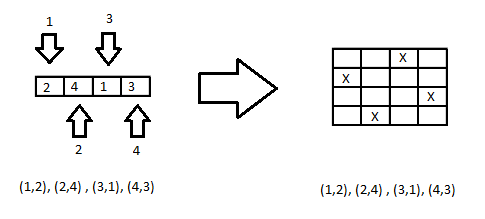
\includegraphics[scale=0.50]{Vectores.png}
%\includegraphics[width=6cm]{../imagenes/general.png}
\caption{Representación de tablero en vector solución (columna,fila)}
\label{foto}
\end{figure}

El proceso de validación se da mediante las “coordenadas” o posiciones que representa la posible lista solución, ya que el entero dentro de una posición x dentro de la lista representa la fila, simplemente verificamos que ningún elemento dentro de la lista se repita, y como posición de la lista representa la columna, nunca habrá que preocuparse porque esta se repita. Para el caso de la verificación en diagonal evaluamos conforme insertarnos en la lista solución, el nuevo elemento no debería estar en una diagonal perteneciente a otra reina, por lo que comparamos el elemento por insertar contra todos los elementos anteriores de la lista, basando el calculo en la propiedad de que entre 2 coordenadas de una misma diagonal existe un N de diferencia para $x_1,x_2$ y $y_1,y_2$ por lo que la comparación: $|x_1 – x_2| == |y_1 – y_2|$  nos dice si se encuentra en la misma diagonal o no.

\begin{figure}[htp]
\centering
\graphicspath{ {imagenes/} }
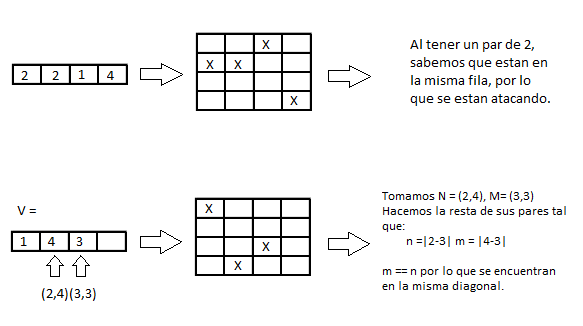
\includegraphics[scale=0.50]{validaciones.png}
%\includegraphics[width=6cm]{../imagenes/general.png}
\caption{Validación por filas y diagonales}
\label{foto}
\end{figure}

Con el fin de explorar todas las posibilidades creamos una lista de tamaño 1 que contiene como único elemento el 1, haciendo referencia a que la reina se encuentra en la posición (1,1) del tablero, luego debemos evaluar todas las posibilidades de una lista de tamaño 2, por lo que agregamos un elemento a la lista en la posición 2, con el numero 1 en dicha posición,  validamos si el vector es valido y como podemos observar tenemos las posiciones (1,1) y (2,1) lo que nos indica que es invalido ya que están en la misma fila, así que haciendo uso del backtracking regresamos al estado anterior el cual era una lista con un 1 como único elemento, y ahora en vez de agregar un 1 continuamos con un 2, por lo que ahora tendríamos una lista con las posiciones (1,1) y (2,2) el cual tampoco es una opción valida ya que dichas posiciones están en la misma diagonal, nuevamente se hace el paso hacia atrás y se agrega a la lista un 3 por lo que ahora tenemos las posiciones (1,1) y (2,3) la cual es una opción valida para continuar, por lo que agregamos nuevamente un 1 a la lista por lo que tendríamos las posiciones (1,1), (2,3) y (1,1), este proceso se repite para N columnas y N filas por lo que, cuando tengamos una lista de tamaño N y sea una opción valida, representara una lista solución. Se podría decir que el proceso de backtracking arma todas las combinaciones de 1 a $N$ posibles de una lista solución de manera controlada, ya que en muchos de los casos, se interrumpe la operación cuando la combinación, o la porción combinacional es invalida.

\begin{figure}[htp]
\centering
\graphicspath{ {imagenes/} }
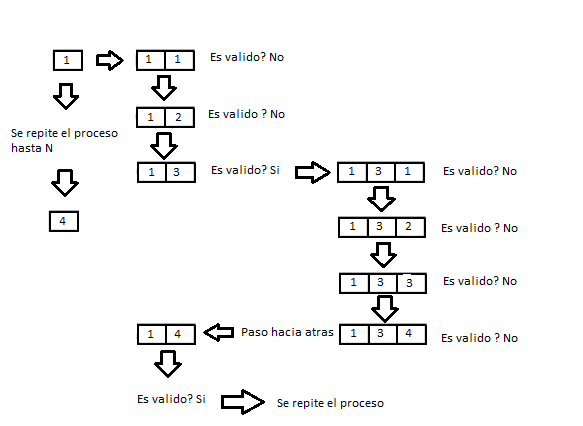
\includegraphics[scale=0.60]{analisisv.png}
%\includegraphics[width=6cm]{../imagenes/general.png}
\caption{Proceso de construcción de una lista solución}
\label{foto}
\end{figure}

\pagebreak
\item  \textbf{Erlang Algoritmos Genéticos} \\

Para describir la solución de algoritmos genéticos, primero es importante definir algunos conceptos básicos en términos del problema para que esta explicación sea más entendible. 
\begin{itemize}
\item Algoritmo genético: es hacer uso de mecanismos que simulan la evolución de las especies de la biología para formular los pasos que describen la búsqueda de una solución a un problema concreto, es una técnica de inteligencia artificial inspirada en la idea de que sobrevive el mejor adaptado a las condiciones.
\item N: número de reinas sobre las que el algoritmo genético va a buscar una solución, su dominio son los números naturales mayores a 3.
\item Cromosomas: un número que abarca de 1 a N, representa una fila donde se encuentra la reina en relación al tablero.
\item Individuo: es una estructura de datos que representa la posición de las N reinas en el tablero, esta compuesto por N cromosomas.
\item Población: estructura de datos que representa la cantidad de individuos sobre los cuales se realiza el algoritmo génetico, para la solución esta dada una población de 4 * N.
\item Elitismo: técnica utilizada, cuando se resuelve un problema con la metodología generacional, en la cual se asegura la sobrevivencia del mejor individuo haciendo que esté presente en la siguiente generación para así no perder la buenas caracteristicas del mismo. 
\item Cruces: es el proceso en el cuál los individuos de una población se cruzan para generar una nueva generación, este cruce está dado de forma aleatoria entre los miembros de la población de la población eso sí con una técnica de selección la cual favorece a los mejor calificación en la función fitness.
\item Función fitness: es un función que $"evalua"$ a los individuos de la población y conforme a sus características les otorga mejor o peor calificación, en términos del problema, dicha calificación esta dada de acuerdo a cuantas veces hay colisiones entre cromosomas, entre menores colisiones, mejores probalidades de perdurar. 
\item Generaciones: son el producto de los cruces de las población, entre más generaciones haya se espera que sea más precisa la aproximación a la respuesta correcta.
\item Mutación: proceso por el cual un crosoma es alterado, se ha trabajado con un 5\% de probalidad de mutación y la estrategia utilizada se basa en escoger dos posiciones de los cromosomas del individuo e intercambiar dichas posiciones, esto con el fin de preservar el fitness que fue calculado para dicho individuo.
\end{itemize}
Una vez entendido los conceptos esenciales para el algoritmo genético, es posible arrancar con la explicación técnica que ha llevado acabo para dar una solución al problema ya mencionado. Se han implementado una serie de funciones primordiales, dichas funciones comprenden:
\begin{enumerate}
\item \textbf{Inicialización de población}: este es el primer paso del algoritmo diseñado, se encarga de inicializar una población en base al parámetro N, que hace referencia al número de reinas, para este caso se ha utilizado una población de tamaño fijo, dado por N * 4, dicha población se presenta es una lista de tamaño 16, donde cado uno de sus elementos posee N genes diferentes, que corresponden a las posiciones de las filas en relación al tablero de ajedrez. La inicialización de esta población se ha realizado haciendo uso de las siguientes funciones:
\begin{verbatim}
poblacion(N) when is_integer(N) -> poblacion(N, N * 4, []).
poblacion(_, 0, R) -> R;
poblacion(N, C, R) -> poblacion(N, C-1, [poblacion_aux(N)|R]).
\end{verbatim} 
\begin{verbatim}
poblacion_aux(N) -> mezclar(lists:seq(1, N)).
\end{verbatim}  
\begin{verbatim}
mezclar(L) when is_list(L) -> 
[Y||{_,Y} <- lists:sort([ {rand:uniform(), N} || N <- L])].
\end{verbatim}  
Estas tres funciones generan una estructura de datos que contiene 16 individuos, compuestos por genes de 1 a N. La salida en consola al ejecutar esta función se ve de la siguiente forma:
\begin{figure}[htp]
\centering
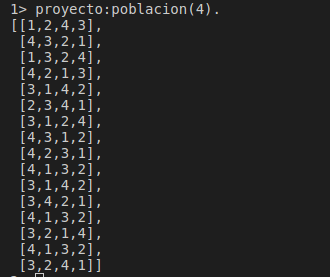
\includegraphics[width=6cm]{imagenes/g1.png} 
\caption{Población generada para un N = 4}
\label{foto}
\end{figure}

\item \textbf{Cálculo de fitness}: esta función es fundamental es el desempeño del algoritmo, se encarga de evaluar todas los genes(posiciones) de un invidividuo para poder determinar que tan apto es con respecto a la necesidad del problema, que ninguna posición de la reina ataque a otra reina. Para este caso el valor de la función se encuentra dado por el número de colisiones o ataques presentes en los genes de un individuo en particular. A menor cantidad de ataques mejor calificado se encuentra el individuo y sus probabilidades de poder existiendo son mayores.
\begin{verbatim}
aptitud(L, N, C) when N > 3 -> lists:reverse(aptitud(L, N, C, [])).
aptitud([], _, 0, R) -> R;
aptitud([H|T], N, C, R) -> aptitud(T, N, C-1, [suma_colisiones(H,N)|R] ).
\end{verbatim}
\begin{verbatim}
suma_colisiones(L, N) -> suma_colisiones(L, 0, N, 0).
suma_colisiones(_, N, N, R) -> R;
suma_colisiones(L, I, N, R) -> suma_colisiones(L, I+1, N, f1(L, N, I+1) + R).
\end{verbatim}
\item \textbf{Crossover}: es la función más importante del algoritmo, para cada par de padres que se cruzan, se elige un punto que  tiene la forma N/2, intentando de esta forma escoger de manera equitativa la cantidad de ambos padres, una vez escogido este punto se unen los genes del primer padre de 1 hasta N/2, y luego se unen los del segundo padre de N/2 a N.
\begin{verbatim}
cruces(L, E, N, C) -> cruce(L, N, C-1, [E]).
cruce(_, _, 0, R) -> lists:reverse(R);
cruce(L, N, C, R) ->  cruce(L, N, C-1, [cruce_aux(L, N, N*4)|R]).
\end{verbatim}
\begin{verbatim}
cruce_aux(L, N, C) -> X1 = rand:uniform(C),
                      X2 = rand:uniform(C), 
                      padres(L, N, X1, X2).
\end{verbatim}
Para poder visualizarlo de una mejor manera, se puede apreciar la siguiente imagen:
\begin{figure}[htp]
\centering
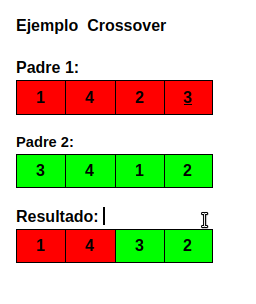
\includegraphics[width=6cm]{imagenes/g2.png} 
\caption{Crossover implementado}
\label{foto}
\end{figure}
\newpage
\item \textbf{Mutación}: la función de mutación se encarga en alterar el orden del los genes de un individuo. Se compone de las siguientes funciones:
\begin{verbatim}
mutacion(P, N) ->  Gen1 = rand:uniform(N),
                   Gen2 = rand:uniform(N),
                   mutar(lists:nth(Gen1, P), lists:nth(Gen2, P), P).
\end{verbatim}
\begin{verbatim}
mutar(Gen1, Gen1, List) -> List;
mutar(Gen1, Gen2, List) -> {P1, P2} = {min(Gen1,Gen2), max(Gen1,Gen2)},
                           {L1, [Elem1 | T1]} = lists:split(P1-1, List),
                           {L2, [Elem2 | L3]} = lists:split(P2-P1-1, T1), 
                           lists:append([L1, [Elem2], L2, [Elem1], L3]).
\end{verbatim}
 Su trabajo es muy sencillo, básicamente se genera un número aleatorio dentro de 0 a 1, si ese número de encuentra dentro del porcentaje de mutación utilizado(5\%) se genera una alteración de dos genes que son escogidos también de manera aleatoria, pero su espacio de posibles valores toma de 1 a N, tenemos entonces: \\
 \begin{figure}[htp]
\centering
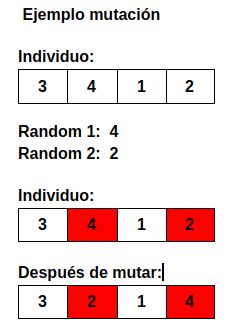
\includegraphics[width=6cm]{imagenes/g3.png} 
\caption{Ejemplo de mutación implementada}
\label{foto}
\end{figure}
\newpage
En la imagen anterior podemos ver un sencillo ejemplo de como trabaja la función, de un individuo en particular se generan dos valores aleatorios, sucede un intercambio de estos valores y el resultado es un nuevo individuo que puede ser favorecido o no por la mutación. \\
La mutación sucede en la función de cruces descrita previamemte, una vez que se ha generado un nuevo individuo, se genera un valor aleatorio que determina si corresponde la aplicación de mutación. 

\item \textbf{Función principal}: es la función controladora de la ejecución del programa, se encarga de utilizar todas las funciones que se han explicado anteriormente, determina cuando se ha encontrado una solución y se encarga de llamar a funciones auxiliares que se encargan de imprimir la solución encontrada, cabe destacar que este algoritmo finaliza su ejecución una vez que se encuentra una solución. La función es:
\begin{verbatim}
geneticosNReinas(N) when N > 3 -> 
                    Poblacion = poblacion(N),
                    calcular(?MAX_CRUCES, Poblacion, N, N*4).
\end{verbatim}
\begin{verbatim}
calcular(0, _, _, _) -> [];
calcular(C, P, N, C) -> A = aptitud(P, N, C),
                        Min = trunc(lists:min(A)),      
                        Pos = min_pos(A, Min, 1),
                        Elite = lists:nth(Pos, P),
                        case Min == 0 of
                        true -> 
                             mostrarSolucion(Elite, N, N, C, []);
                        false -> 
                             eliteActual(Elite, C),
                             N_P = cruces(P, Elite, N, C),
                             calcular(C-1, N_P, N, C) end.
\end{verbatim}
Aquí se puede apreciar el ciclo de vida del algoritmo, cabe resaltar que la cantidad máxima de cruces para el algoritmo quedó definido en 1000 cruces, por lo que si efectuados 1000 cruces no hay una solución de resolución finalizara la ejecución. 
\end{enumerate}
\end{enumerate}
\pagebreak
\section{Resultados de las pruebas}

Tomando en cuenta el hecho de que el algoritmo de backtracking está diseñado para obtener todas las soluciones posibles y el de genéticos solamente una solución cada vez que este se corre, decidimos realizar 2 tipos de pruebas distintas, tomando en cuenta N = 5...15, donde una de las pruebas se realizó con el fin de obtener una única solución y otra donde se calcularon 5 soluciones por cada N reinas, esto para entrar en la fortaleza del algoritmo genético y también aprovechar la propiedad del backtracking para encontrar mas de una solución, sin embargo cabe destacar que no se hicieron pruebas solicitando mas de 5 soluciones ya que para el algoritmo genetico existe una probabilidad de que no encuentre una solucion en su ejecucion debido al agotamiento de cruces establecidos, el cual aunque sea un valor muy grande, existe la posibilidad de que se agote y no de respuesta valida. Los resultados del tiempo de ejecución pueden apreciarse en la figura 5 y 6.  \\

\begin{figure}[htp]
\centering
\graphicspath{ {imagenes/} }
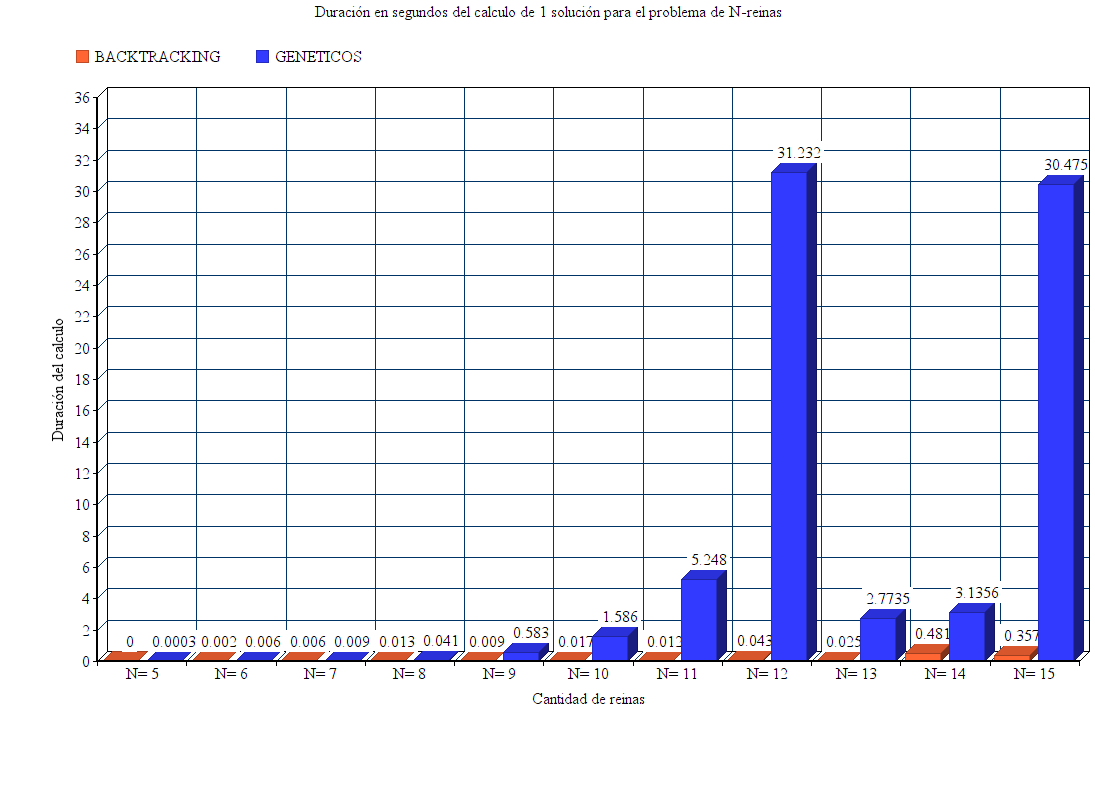
\includegraphics[scale=0.60]{analisis1.png}
%\includegraphics[width=6cm]{../imagenes/general.png}
\caption{Grafico con tiempos de corrida para una solución}
\label{foto}
\end{figure}
\pagebreak

\begin{figure}[htp]
\centering
\graphicspath{ {imagenes/} }
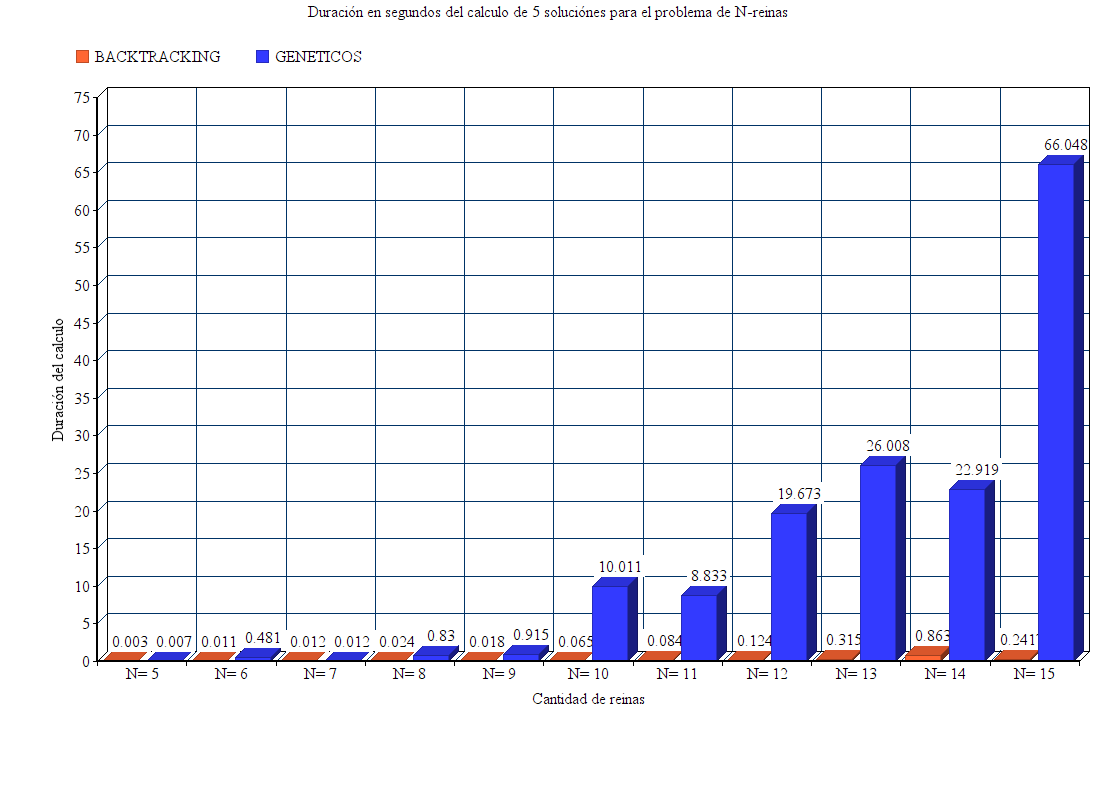
\includegraphics[scale=0.60]{analisis5.png}
%\includegraphics[width=6cm]{../imagenes/general.png}
\caption{Grafico con tiempos de corrida para 5 soluciónes}
\label{foto}
\end{figure}

Basándonos solamente en lo que indican las graficas podemos concluir que la implementación con algoritmos genéticos, es mas lenta que la implementación con backtracking, está ultima pudo calcular 1 solución para 15 reinas en menos de 1 segundo, esto en parte se debe a que el escenario propuesto es ventajoso para el backtracking, esto debido a la manera sistemática en la que calcula la solución, sin embargo, para un N mayor a 20, incluso una solución es muy difícil de obtener, siendo 25 el limite de reinas para el que logramos obtener una única solución.

También es importante mencionar el hecho de que el algoritmos está diseñado para calcular todas las posibles soluciones por lo que calcular una cantidad limitada de estas, mejorará su desempeño, si se desease calcular todas las posibilidades, este algoritmo comenzaría a quedarse corto desde el calculo para n = 12, el cual tiene 14200 soluciones, y que tomó 3,8 minutos para ser resuelto, En cambio, la implementación del algoritmo genético está diseñado para obtener una única solución, trabajando en un modelo que simula la evolución y que utiliza la aleatoriedad como un punto importante para la evolución constaste de las posibles soluciones, esto implica que existe una probabilidad mucho mayor de obtener una solución para cualquier N reinas incluyendo las mayores a 25, punto de muerte en sentido de optimización para el algoritmo de backtracking.
Respecto a la velocidad con la que se encuentra una única solución, para el algoritmo de backtracking, suele ser constante o muy similar para un mismo valor N, esto debido a que siempre se calculara primero la misma solución en el mismo recorrido sistemático sobre la metodología de la implementación  en cada ejecución del programa, ademas no es usual obtener un mejor tiempo para una solución N+1, esto solo es capaz de suceder para N menores a 5, a partir de esto los tiempos de ejecución aumentan significativamente entre soluciones. Por otro lado el algoritmo genético, debido al nivel de aleatoriedad que este implementa, no garantiza que el resultado sea el mismo cada vez que se ejecuta, ni tampoco su tiempo de ejecución, a como puede encontrar una solución en fracción de segundo, puede tardar una cantidad de tiempo significativa, y esto se puede observar al ejecutar M veces el programa para la misma cantidad de reinas,  incluso mediante la grafica para 1 solución podemos observar como el tiempo de ejecución para 12 reinas es mayor que el de 15, lo cual nunca sucede para backtracking.
Con estas observaciones podemos concluir que el algoritmo de backtracking es superior al algoritmo genético cuando lo que deseamos es obtener una solución para un N menor a 25,  e incluso para obtener todas sus soluciones cuando el N es mas pequeño que 13, incluyendo el beneficio para una cierta situación de que las soluciones serán siempre las mismas, por otro lado el algoritmo genético es una opción mas viable para N muy grandes, también cuando se desea observar una solución distinta para cada ejecución sin necesidad de tomarse la molestia de calcular todas las respuestas posibles.

\pagebreak
\section{Conclusiones}
Tomando en cuenta lo expuesto, podemos concluir que la implementación de ambos algoritmos es completamente funcional, mas no optima en todas las situaciones para las que esta pueda ser utilizada, esto debido a sus enfoques de implementación y el sistema utilizado por cada algoritmo para encontrar la solución, así mismo un punto importante es la facilidad de implementación de dichos algoritmos, en la cual el backtracking resulta ser muy sencillo en comparación al algoritmo genético. \\

El calculo sistemático que provee el backtracking resulta en una velocidad mayor y constante, también nos permite tener al alcance todas o unas cuantas  soluciones posibles, las cuales siempre serán las mismas, en el mismo orden, claro, todo esto enfocándonos al calculo de soluciones para una cantidad no muy grande de reinas; Por otro lado, cuando nos referimos a los algoritmos genéticos para la implementación de este problema, podemos mencionar la ventaja superior en el calculo de soluciones para situaciones en las que el numero de soluciones necesarias sea muy pequeña pero la cantidad de reinas sea muy grande, también mencionar el hecho de que su aleatoriedad que aunque altera el tiempo de ejecución para una misma cantidad de reinas,  resulta muy útil cuando se necesitan soluciones distintas para una misma reina.
\\

Refiriéndonos a los lenguajes utilizados, Erlang posee una sintaxis mucho mas sencilla de entender y utilizar, especialmente para la implementación del algoritmo genético, ya que este necesita manejar aleatoriedad, construcción de listas e interpretación de evaluaciones constantes, para conseguir la metodología evolutiva, en Scheme esto no es algo muy sencillo de lograr, pero la utilidad que posee para utilizar la recursividad resultó muy útil para la implementación del backtracking, claro, dejando de lado la complejidad que este posee en su sintaxis y comprensión.
\\
\newpage
\section{Aprendizajes}
\bigskip
	Como parte de los aprendizajes que se han logrado obtener durante el desarollo del proyecto NQueens resaltan los  siguientes:
	\begin{enumerate}
		\item Uno de los retos cuando fue asignado el proyecto era poder cambiar la forma de pensamiento, poder desarrollar un solución óptima no solo requería entender el problema, había que interiorizar de buena manera la lógica del paradigma sobre el cual iba a estar construida dicha solución. Por otra parte, eran dos lenguajes distintos, pese a trabajar bajo el mismo paradigma funcional, presentaban características de sintaxis muy distintas entre ellos. De manera de aprendizaje es posible destacar lo importante de la investigación por parte de los miembros del proyecto, cada uno se comprometío a investigar y poder entregar una solución, lo cual fue muy beneficioso para el bien del proyecto.
	\item Conocimiento de la estrategia de backtracking, como puede ser aplicado para resolver múltiples problemas y que en lenguajes funcionales como Scheme resultan ser muy potentes. Se pudo observar que mediante esta estrategia es posible obtener  todo el árbol de soluciones de un problema, de esta forma mediante el uso de otra técnica en conjunto con esta se puede encontrar la solución más óptima a un problema.
	\item Primer acercamiento a tecnología relacionadas a inteligencia artificial, el tema de algoritmos genéticos describe los procesos que rigen la vida de los seres vivos, y como dichos procesos pueden ser aplicados en resolver problemas que en principio no tendrían ninguna relación. Es sencillamente interesante poder plasmar mediante código de programación la forma en como la vida misma ha evolucionado durante millones de años. Este tipo de ejercicios abre una puerta por la cual el estudiante puede empezar a conocer nuevas aplicaciones de tecnologías, tanto en el campo de investigación como su aplicación directa sobre distintos problemas de la vida cotidiana.
	 \item Uso de nuevas herramientas, no solo los lenguajes sobre los cuales han sido desarolladas las soluciones, también se fortalece el conocimiento de Latex como una poderosa herramienta de documentación profesional.
	\end{enumerate}
\newpage
\begin{thebibliography}{20}
\bibitem{Genetic vs Backtracking}{Arkar, U., Nag, S. 2017. An Adaptive Genetic Algorithm for Solving N-Queens Problem. [online]. Available at: https://arxiv.org/abs/1802.02006}
\bibitem{a}{Canela, A y González, B. 2014. Ilustración representativa de la metodología backtracking en el problema de las N-reinas. [online] Available at: http://estructuradedatos2backtracking.blogspot.com/2014/}
\bibitem{a}{Canela, A y González, B. 2014. BACKTRACKING [online]. Available: http://estructuradedatos2backtracking.blogspot.com/2014/ }
\bibitem{a}{Ecured.cu. 2020. Scheme - Ecured. [online] Available at: https://www.ecured.cu/Scheme }
\bibitem{a}{Ecured.cu. 2020. Erlang - Ecured. [online] Available at: https://www.ecured.cu/Erlang }
\bibitem{a}{Kora, Padmavathi, Yadlapalli, Priyanka. 2017. Crossover Operators in Genetic Algorithms: A Review. International Journal of Computer Applications.  [online]. Available at: https://www.researchgate.net/publication/315175882/}
\bibitem{Genetic vs Backtracking}{Medium. 2020. Genetic Algorithm Vs. Backtracking: N-Queen Problem. [online] Available at: https://towardsdatascience.com/genetic-algorithm-vs-backtracking-n-queen-problem-cdf38e15d73f}
\bibitem{Genetic vs Backtracking}{Notxor.nueva-actitud.org. 2020. Mis Impresiones Sobre Erlang - Notxor Tiene Un Blog. [online] Available at: https://notxor.nueva-actitud.org/blog/2020/07/25/mis-impresiones-sobre-erlang/}
\bibitem{Genetic vs Backtracking}{Rubicite.com. 2020. Order 1 Crossover Operator Tutorial. [online]. Available at: http://www.rubicite.com/Tutorials/GeneticAlgorithms/CrossoverOperators/Order1CrossoverOperator.aspx}
\bibitem{Genetic vs Backtracking}{Thede, S. 2020. A Generalized Parallel Genetic Algorithm In Erlang. [online]. Available at: https://www.academia.edu/16713281/}
\bibitem{Genetic vs Backtracking}{Vanacore, C (2019, mayo 24). “Backtracking and Crossword Puzzles” [online]. Available at: https://medium.com/@vanacorec/backtracking-and-crossword-puzzles-4abe195166f9}

\end{thebibliography}

\end{document}
\end{document}